\section{Results}\label{sect:results}

\begin{itemize}
    \item Images of select cases, demonstrating segmentation process
\end{itemize}

The computed volumes of the prostates from the MR and ARFI imaging data are
presented in Table~\ref{tab:mr_arfi_volumes}.  The subvolumes associated
with the zonal anatomy in each imaging modality was measured
(Figure~\ref{fig:mr_arfi_volumes}(a)), showing an mean overestimation of
total prostate volume of 36.7 $\pm$ 27.9\% by ARFI imaging compared to MR
volumes (Figure~\ref{fig:mr_arfi_volumes}(b)), and a relative
underestimation of the central zone volume relative to the central gland in MR
imaging of -15.3 $\pm$ 13.0 \% (Figure~\ref{fig:mr_arfi_volumes}(c)).

\begin{table}[h!]
\centering
\caption{Comparison of Central Gland / Zone and Total Prostate Volumes in MR T2WI and \textbf{B-mode/}ARFI Imaging}
\begin{tabular}{|l|l|l|l|l|} \hline
{\bf Study Subject} & {\bf MR Central Gland} & {\bf MR Total} & {\bf ARFI Central Gland} & {\bf B-mode Total} \\ 
& {\bf Volume (cm$^3$)} & {\bf Volume (cm$^3$)} & {\bf Volume (cm$^3$)} & {\bf Volume (cm$^3$)} \\ \hline
1 & 12.74 & 24.57 & 14.30 & 19.31 \\ 
2 & 14.26 & 28.51 & 8.37 & 32.90 \\ 
3 & 23.47 & 32.48 & 13.29 & 24.24 \\ 
4 & 17.32 & 32.49 & 10.83 & 28.98 \\ 
5 & 57.56 & 70.95 & 30.37 & 65.55 \\ 
6 & 12.01 & 27.84 & 15.68 & 28.71 \\ 
7 & 8.82 & 19.59 & 11.78 & 23.32 \\ 
8 & 10.97 & 21.28 & 16.02 & 27.72 \\ 
9 & 13.63 & 20.75 & 19.28 & 27.84 \\ 
10 & 23.58 & 36.11 & 33.50 & 58.07 \\ 
11 & 16.57 & 27.33 & 25.22 & 32.78 \\ 
12 & 25.38 & 49.21 & 18.14 & 50.35 \\ 
13 & 9.25 & 26.36 & 6.14 & 32.66 \\ 
14 & 14.79 & 23.36 & 11.60 & 20.68 \\ 
15 & 17.87 & 35.37 & 10.15 & 35.29 \\ 
16 & 33.32 & 48.50 & 19.31 & 31.76 \\ 

\hline
\end{tabular}
\label{tab:mr_arfi_volumes}
\end{table}


\begin{figure}[htb!]
\centering
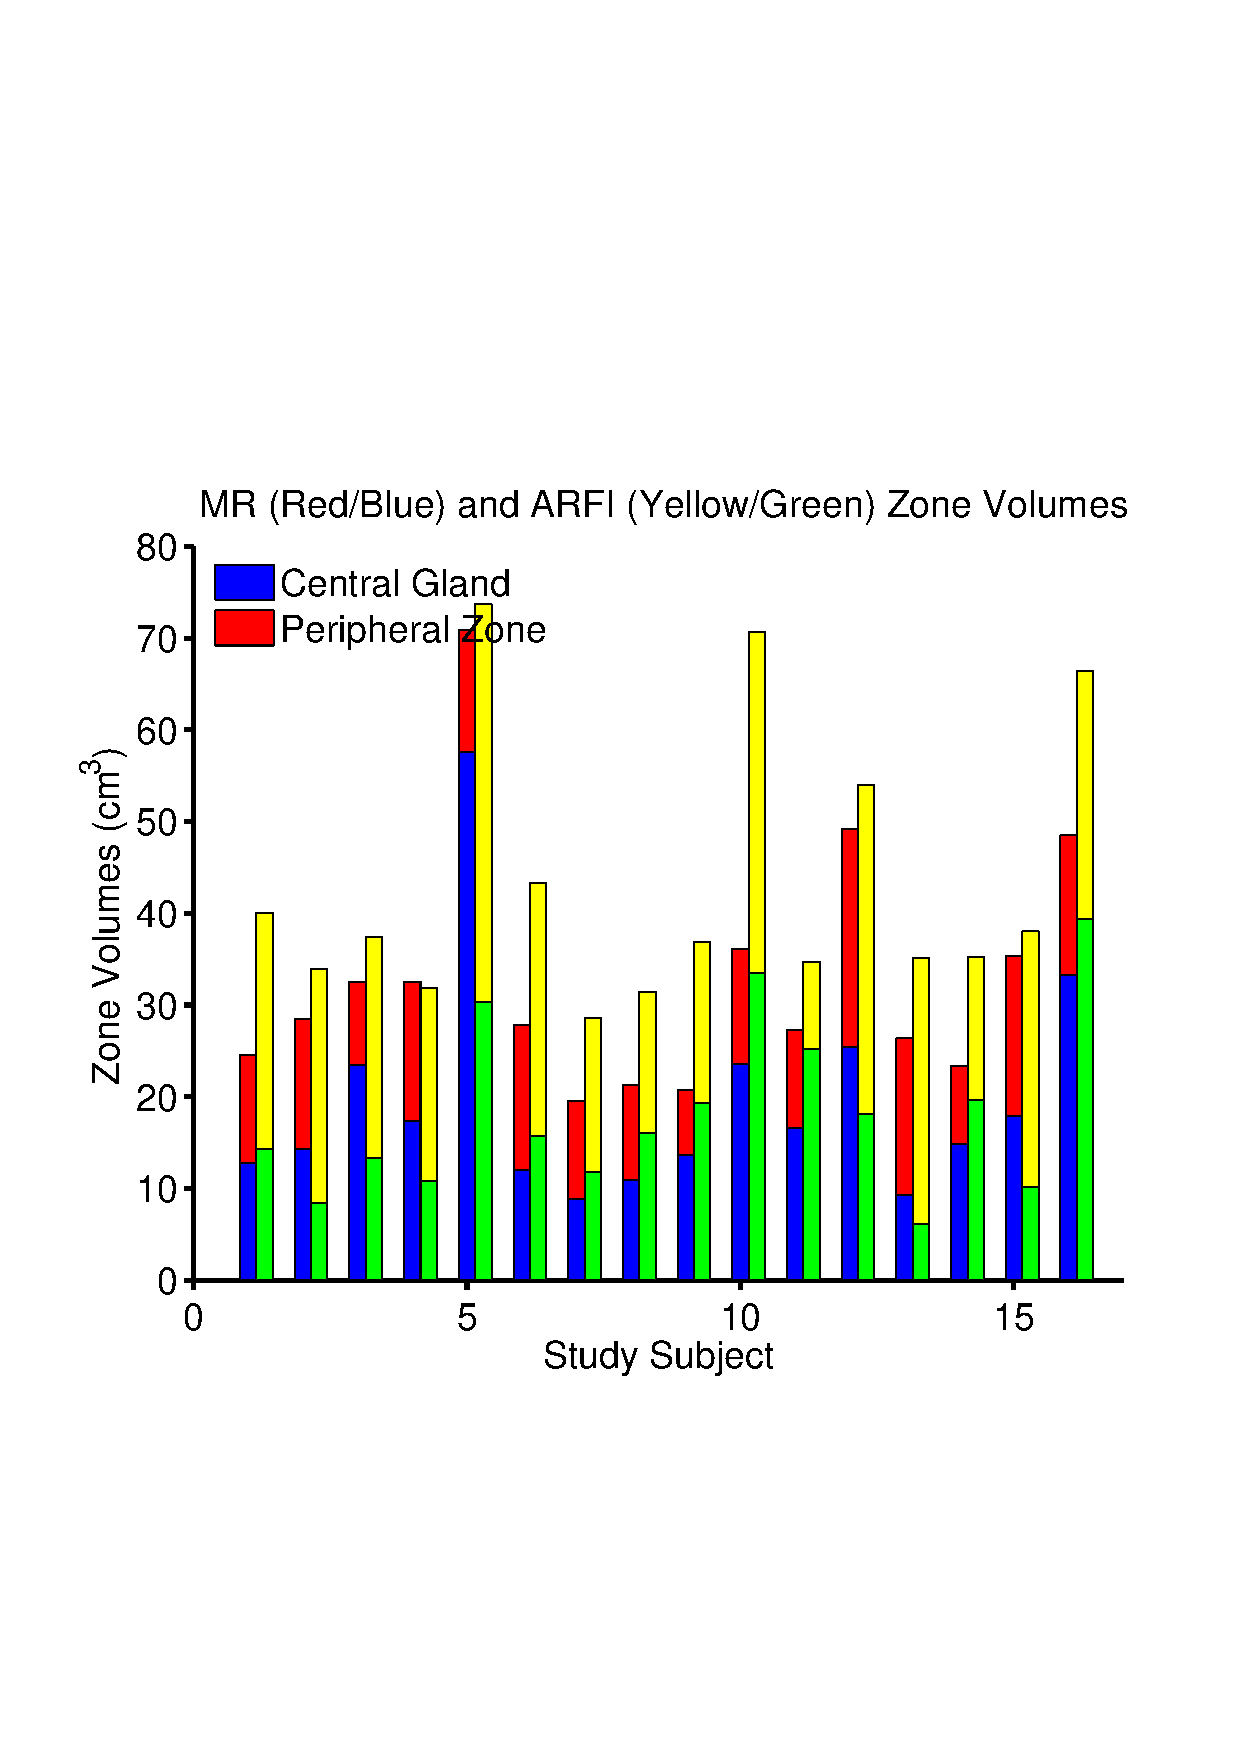
\includegraphics[width=0.5\linewidth]{figs/mr_arfi_volumes.pdf}
\caption{MR and ARFI volumes - need more text here}
\label{fig:mr_arfi_volumes} 
\end{figure}


Weights and axis measurements from the gross pathology processing of the
excised prostates were collected (Table~\ref{tab:path_data}), and using the
axis measurements (lateral-to-lateral, anterior-to-posterior, and
apex-to-base), the prostate volume was approximated as a tri-axial ellipsoid,
and its volume was estimated.

\begin{table}
\centering
\caption{Pathology Prostate Gross Specimen Metrics}
\begin{tabular}{|l|l|l|l|l|l|} \hline
{\bf Study } & {\bf Weight} & {\bf Lat-Lat} & {\bf Anterior-} & {\bf Apex-Base} & {\bf Ellipsoidal} \\
{\bf Subject} & {\bf (g)} & {\bf (cm)} & {\bf Posterior (cm)} & {\bf (cm)} & {\bf Volume (cm$^3$)} \\ \hline
1 & 37. & 4.3 & 4.0 & 2.9 & 26.10 \\ 
2 & 52. & 4.5 & 3.5 & 3.5 & 28.85 \\ 
3 & 38. & 4.5 & 4.0 & 3.7 & 34.85 \\ 
4 & 84. & 7.0 & 6.5 & 6.0 & 142.87 \\ 
5 & 72. & 6.6 & 4.3 & 3.0 & 44.56 \\ 
6 & 49. & 4.9 & 4.4 & 3.4 & 38.36 \\ 
7 & 25. & 3.7 & 3.7 & 3.2 & 22.93 \\ 
8 & 27. & 4.2 & 3.1 & 2.7 & 18.40 \\ 
9 & 28. & 4.4 & 3.7 & 3.2 & 27.26 \\ 
10 & 42. & 4.7 & 3.5 & 3.2 & 27.55 \\ 
11 & 38. & 5.4 & 4.0 & 3.3 & 37.30 \\ 
12 & 50. & 5.0 & 4.0 & 3.7 & 38.73 \\ 
13 & 29. & 4.0 & 3.5 & 3.0 & 21.98 \\ 
14 & 27. & 4.5 & 3.0 & 3.0 & 21.20 \\ 
15 & 32. & 4.5 & 3.5 & 3.5 & 28.85 \\ 
16 & 62. & 5.5 & 5.3 & 5.2 & 79.33 \\ 

\hline
\end{tabular}
\label{tab:path_data}
\end{table}


MR and ARFI imaging total prostate volumes were also compared with the weights
and prostate volumes, approximated to be tri-axial ellipsoids, and calculated
from measurements of the prostate semi-principal axes.  Prostate weights were
moderately correlated with estimated pathology ellipsoidal prostate volumes
(Figure~\ref{fig:mr_arfi_weight}(a), R$^2$ = 0.68).  There was moderate
correlation between the prostate weight and the image-reconstructed prostate
volumes (Figure~\ref{fig:mr_arfi_weight}(b), R$^2$ = 0.44 (MR) and 0.21
(ARFI)), though there was weaker correlation with the ellipsoidal approximation
of the measurement prostate volume and the image-recontructed volumens
(Figure~\ref{fig:mr_arfi_weight}(c), R$^2$ = 0.08 (MR) and 0.01 (ARFI)).  

\begin{figure}[htb!]
\centering
\begin{tabular}{lll}
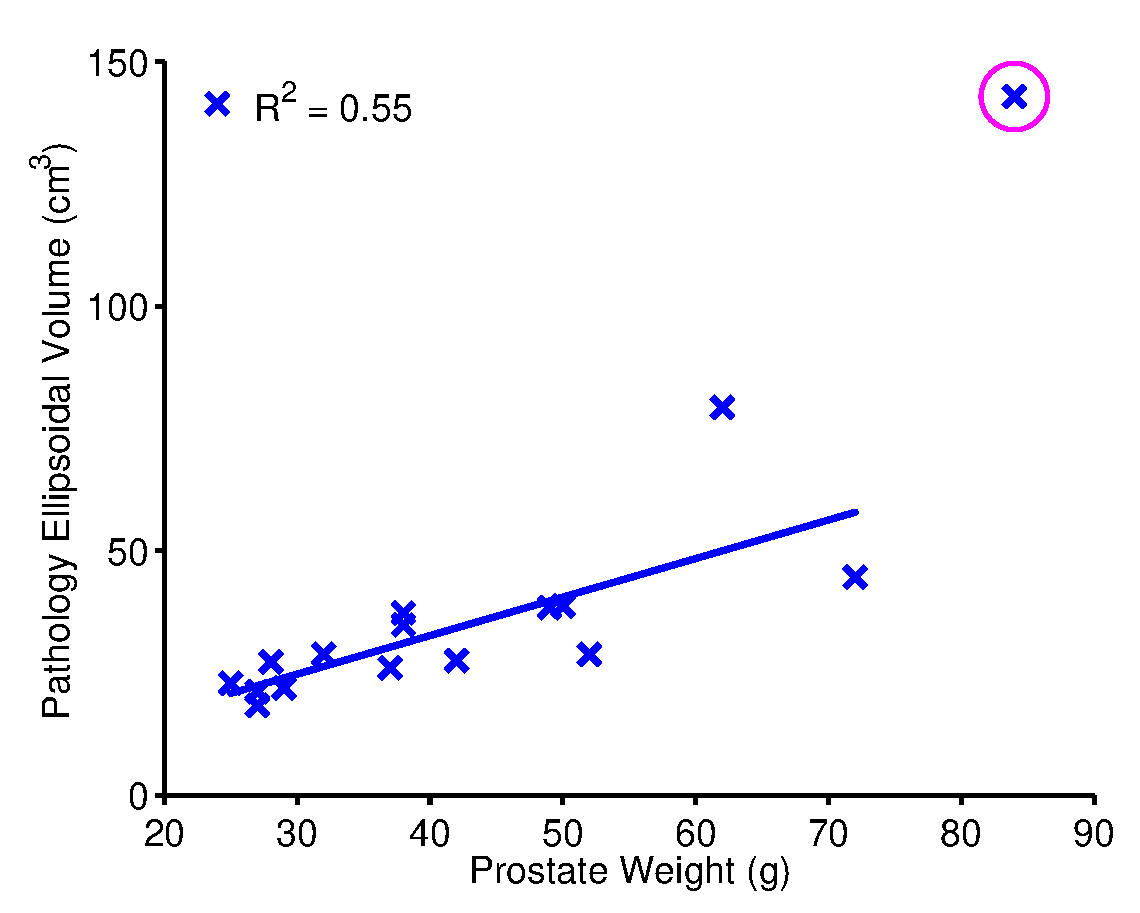
\includegraphics[width=0.3\linewidth]{figs/corr_path_vol_weight_vol} &
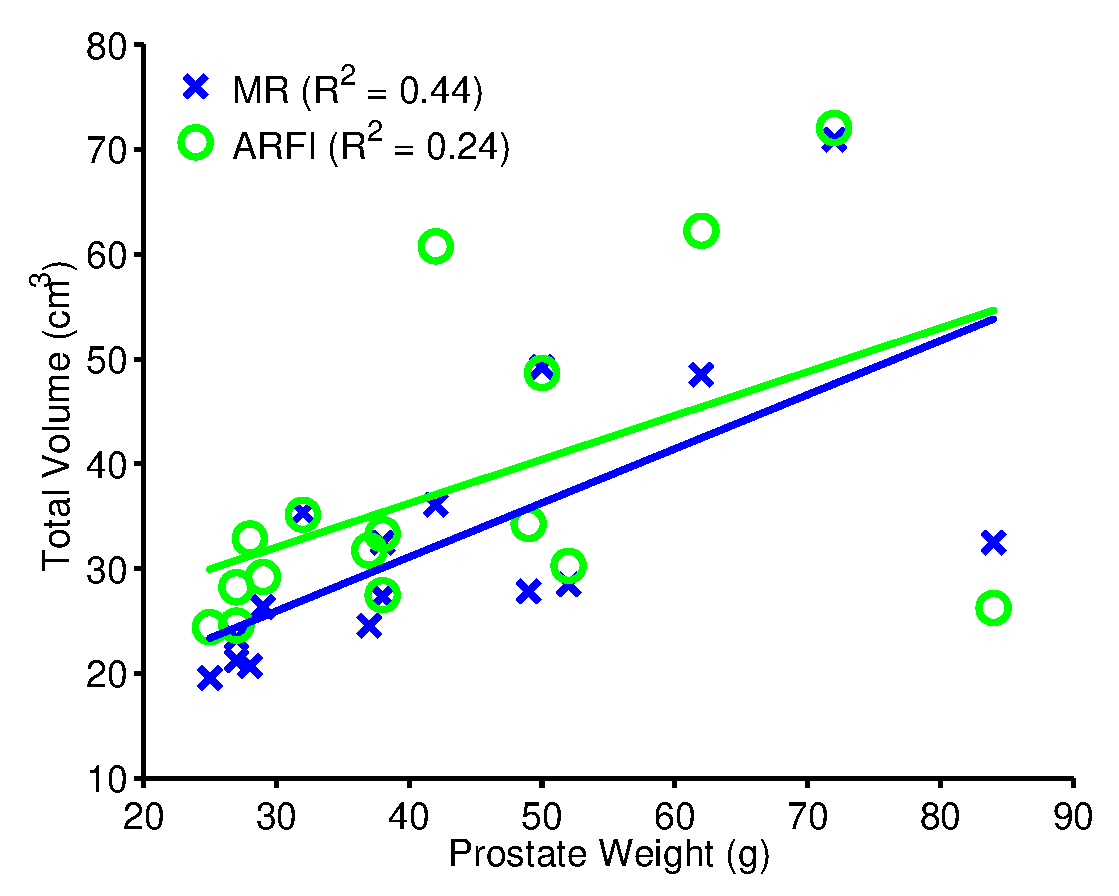
\includegraphics[width=0.3\linewidth]{figs/corr_weight_vol} &
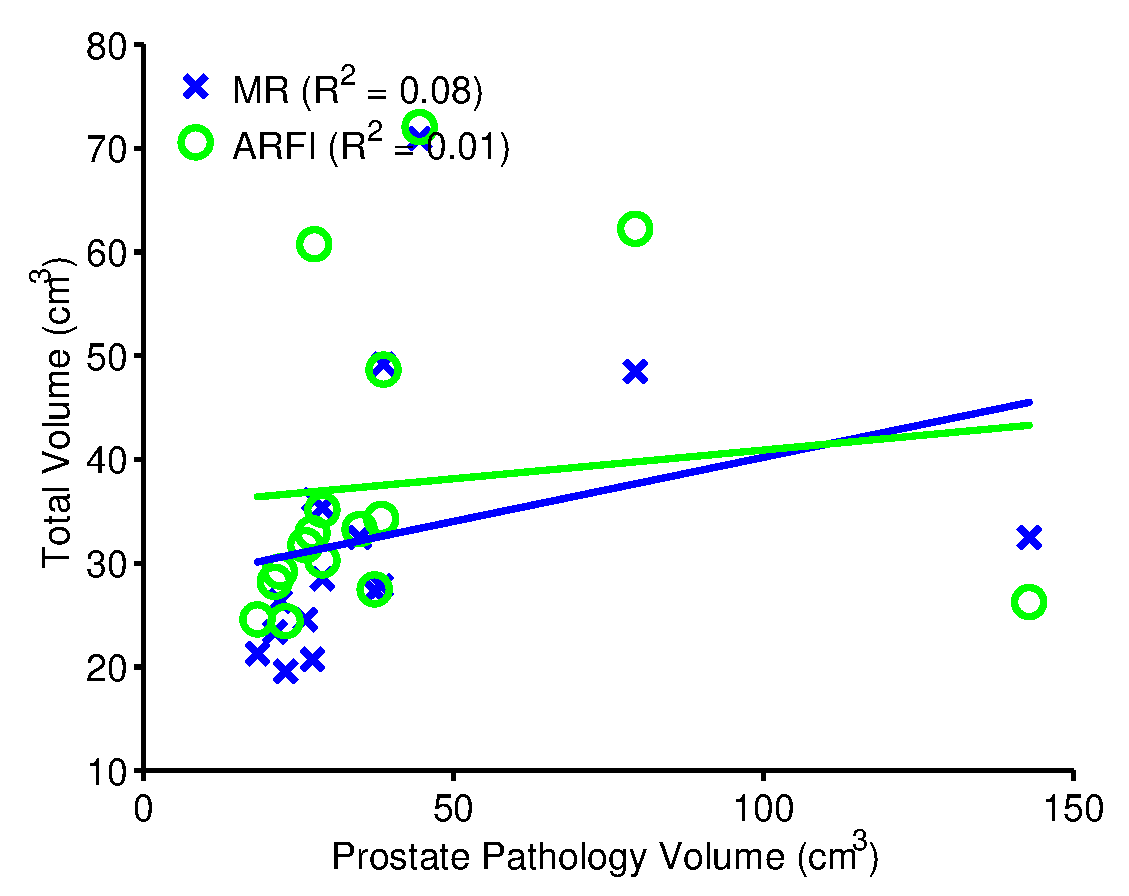
\includegraphics[width=0.3\linewidth]{figs/corr_pathVol_vol} \\
(a) Path Weight : Path Volume & (b) Image Volume : Prostate Weight & (c) Image Volume : Path Volume \\
\end{tabular}
%\begin{tabular}{ll}
%\includegraphics[width=0.3\linewidth]{figs/corr_weight_vol_no4} &
%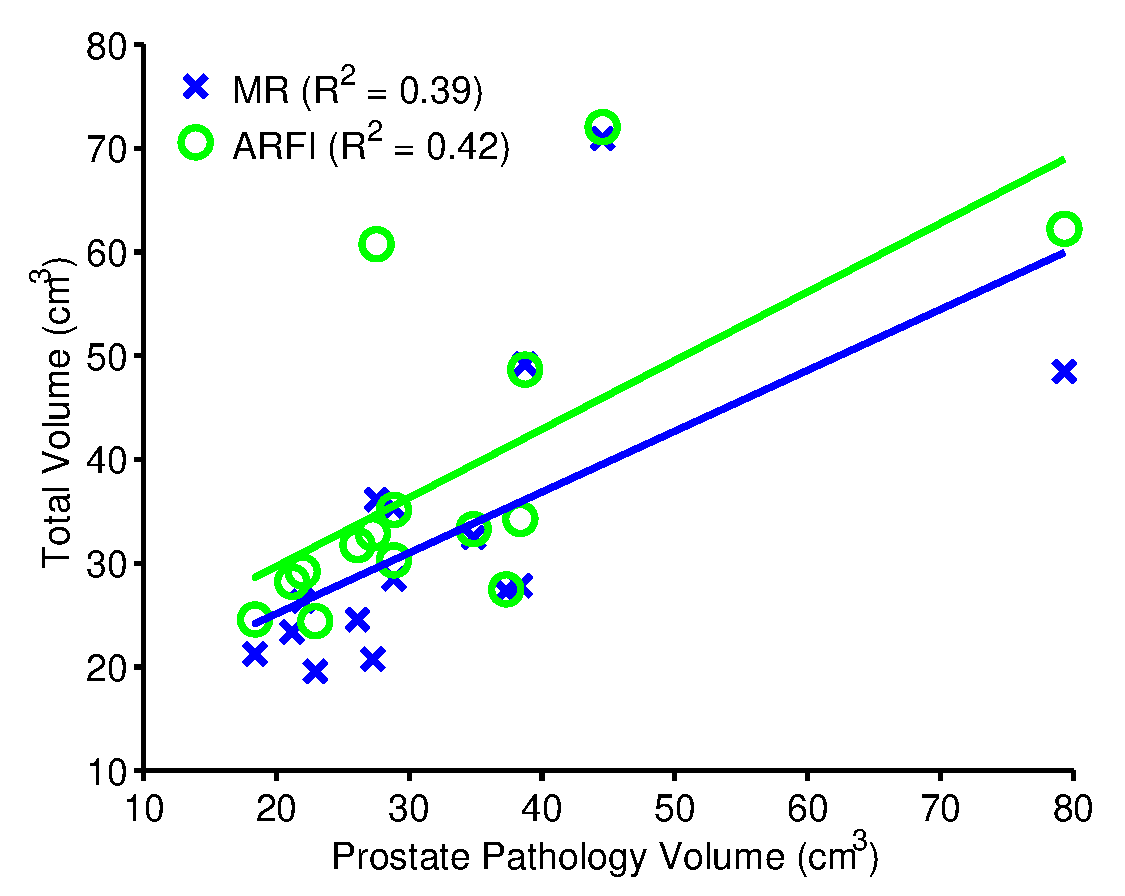
\includegraphics[width=0.3\linewidth]{figs/corr_pathVol_vol_no4} \\
%(d) Image Volume : Prostate Weight (-4) & (e) Image Volume : Path Volume (-4) \\
%\end{tabular}
\caption{Tri-axial pathology measurements were used to make an ellipsoidal
    prostate volume approximation based on gross pathology axis measurements,
    which was moderately well-correlated with the excised prostated weights (a,
    R$^2$ = 0.68).  T2WI MR (blue, X) showed a moderate correlation between the
    reconstructed volumes and prostate weight (R$^2$ = 0.44), while volumes
    reconstructed from ARFI images (green, O) showed weaker correlation (R$^2$
    = 0.21) (b).  Even weaker correlations existed between both T2WI MR and
    ARFI image volumens and approaximated ellipsoidal prostate pathology
    volumes (R$^2$ = 0.08 and 0.01, respectively) (c).  It should be noted in
    these figures that two study subjects had excessively large prostates that
    were difficult to fully capture in imaging (volumes $>$ 60 cm$^3$),
    especially in their anterior region, and they were, therefore, grossly
    underestimated in size.}
\label{fig:mr_arfi_weight}
\end{figure}


While difficult to compare the absolute lengths of the major and minor
anatomical axes of the prostates between the imaging modalities and pathology
due to different geometric distortions during imaging and changes to the organ
after excision, measurements of the prostate dimensions along the three
standard anatomic axes (apex-to-base, lateral-to-lateral, and
anterior-to-posterior) were made (Table~\ref{tab:mr_arfi_axes}), and the
relative ratios of the axes in imaging and pathology for the total prostate
volume were compared (Figure~\ref{fig:mr_arfi_total_axes}), and the relative
ratios of the central gland / zone anatomy were compared for MR and ARFI
imaging (Figure~\ref{fig:mr_arfi_central_axes}).  The mean ratio differences between ARFI imaging, T2WI MR and pathology are compiled in Table~\ref{tab:axis_ratio_over_under}.

\begin{table}
\centering
\caption{Comparison of Central Gland / Zone and Total Prostate Major / Minos Axes in MR T2WI and ARFI Imaging}
\begin{tabular}{|l|l|l|l|l|l|l|l|l|l|l|l|l|} \hline
{\bf Study} & {\bf MR} & {\bf MR} & {\bf MR} & {\bf MR} & {\bf MR} & {\bf MR} & {\bf ARFI} & {\bf ARFI} & {\bf ARFI} & {\bf ARFI} & {\bf ARFI} & {\bf ARFI} \\ 
{\bf Subject} & {\bf CA} & {\bf CL} & {\bf CE} & {\bf TA} & {\bf TL} & {\bf TE} & {\bf CA} & {\bf CL} & {\bf CE} & {\bf TA} & {\bf TL} & {\bf TE} \\
 & {\bf (cm)} & {\bf (cm)} & {\bf (cm)} & {\bf (cm)} & {\bf (cm)} & {\bf (cm)} & {\bf (cm)} & {\bf (cm)} & {\bf (cm)} & {\bf (cm)} & {\bf (cm)} & {\bf (cm)} \\ \hline
1 & 4.12 & 2.90 & 2.45 & 4.12 & 3.80 & 3.09 & 4.34 & 3.51 & 2.28 & 5.26 & 4.94 & 3.14 \\ 
2 & 3.87 & 3.39 & 2.80 & 3.87 & 4.45 & 3.59 & 4.03 & 3.25 & 1.66 & 3.06 & 5.46 & 3.86 \\ 
3 & 4.82 & 3.48 & 3.27 & 5.11 & 4.11 & 3.59 & 4.53 & 3.23 & 2.29 & 4.53 & 4.55 & 3.68 \\ 
4 & 5.35 & 3.08 & 2.87 & 5.36 & 4.45 & 3.37 & 3.82 & 2.62 & 2.35 & 4.18 & 4.63 & 3.66 \\ 
5 & 6.22 & 4.66 & 4.98 & 7.39 & 5.43 & 5.63 & 5.20 & 5.06 & 2.42 & 5.20 & 6.24 & 4.28 \\ 
6 & 5.05 & 3.44 & 3.44 & 5.10 & 4.84 & 3.44 & 4.63 & 3.96 & 2.29 & 4.50 & 5.83 & 3.10 \\ 
7 & 4.47 & 3.33 & 2.26 & 4.72 & 4.44 & 2.58 & 4.77 & 3.42 & 2.40 & 3.92 & 4.80 & 2.84 \\ 
8 & 4.30 & 3.20 & 2.10 & 4.32 & 4.23 & 2.48 & 5.72 & 4.23 & 2.52 & 4.50 & 4.71 & 2.97 \\ 
9 & 3.52 & 3.31 & 2.19 & 3.52 & 4.33 & 2.70 & 4.73 & 4.90 & 2.69 & 4.43 & 5.71 & 3.06 \\ 
10 & 5.24 & 4.43 & 2.69 & 5.23 & 5.15 & 3.37 & 5.02 & 7.19 & 2.20 & 4.85 & 7.46 & 3.20 \\ 
11 & 5.02 & 3.85 & 2.73 & 5.02 & 5.50 & 3.57 & 4.24 & 4.31 & 2.72 & 3.15 & 5.16 & 2.78 \\ 
12 & 4.55 & 3.70 & 3.30 & 4.58 & 5.38 & 4.24 & 4.24 & 4.63 & 2.34 & 3.87 & 6.74 & 3.83 \\ 
13 & 3.40 & 4.03 & 2.01 & 4.08 & 4.72 & 2.94 & 2.84 & 3.29 & 1.91 & 3.89 & 5.31 & 3.46 \\ 
14 & 3.56 & 3.69 & 2.54 & 3.56 & 4.33 & 3.17 & 4.18 & 4.84 & 2.29 & 4.14 & 5.04 & 3.02 \\ 
15 & 4.79 & 4.17 & 2.56 & 4.95 & 4.69 & 3.32 & 5.00 & 3.78 & 3.08 & 4.12 & 5.31 & 3.60 \\ 
16 & 5.11 & 4.60 & 3.11 & 5.12 & 5.62 & 3.71 & 5.03 & 6.14 & 3.13 & 4.61 & 6.23 & 3.52 \\ 

\hline
\end{tabular}
\label{tab:mr_arfi_axes}
\end{table}


\begin{figure}[htb!]
\centering
\begin{tabular}{ccc}
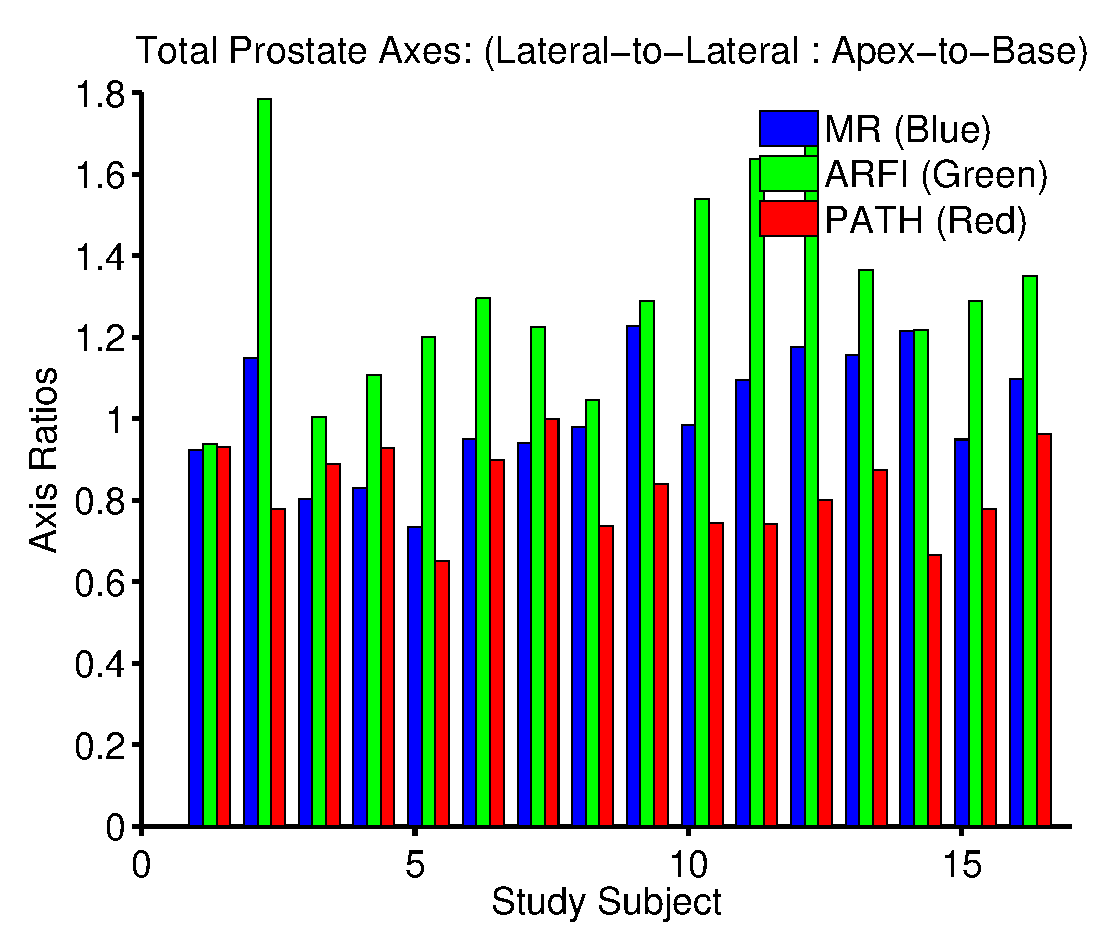
\includegraphics[width=0.3\linewidth]{figs/mr_arfi_total_axes1} &
\includegraphics[width=0.3\linewidth]{figs/mr_arfi_total_axes2} &
\includegraphics[width=0.3\linewidth]{figs/mr_arfi_total_axes3} \\
(a) & (b) & (c) \\
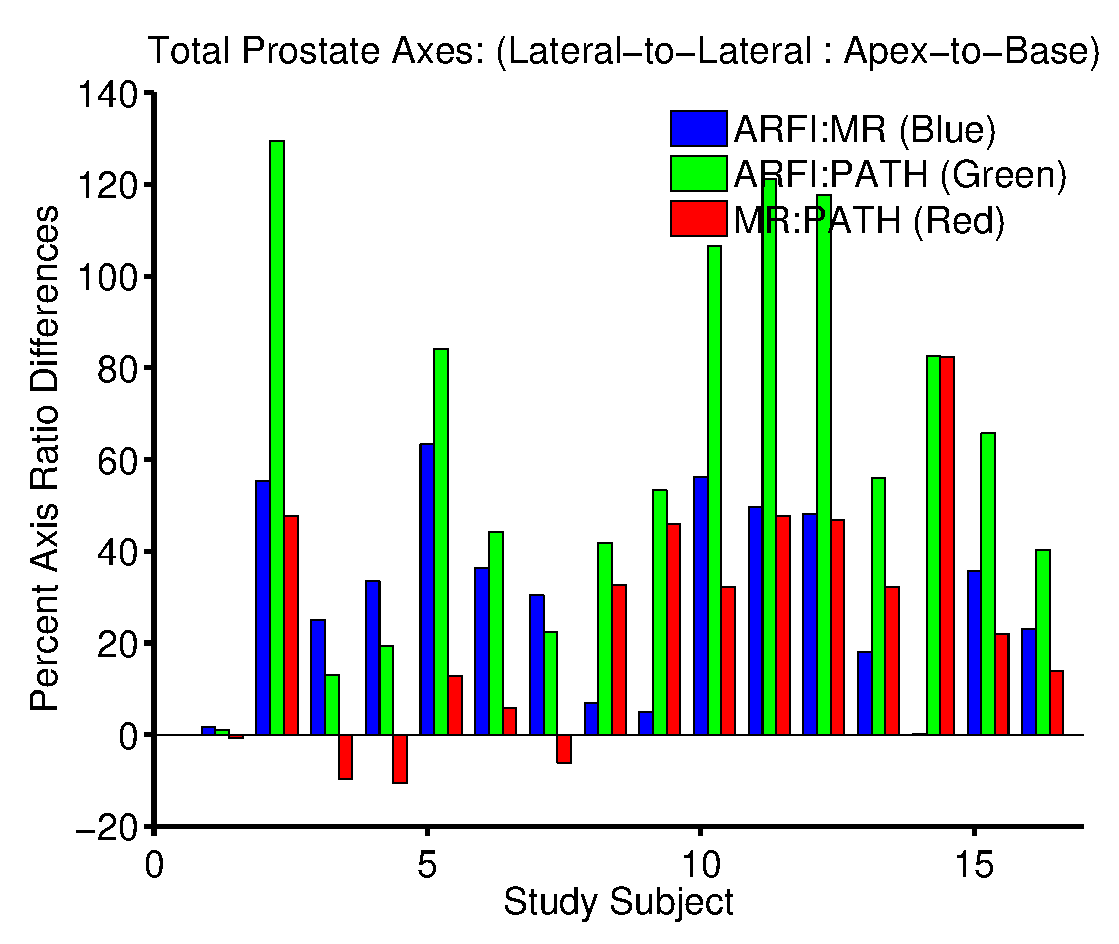
\includegraphics[width=0.3\linewidth]{figs/mr_arfi_total_over_under1} &
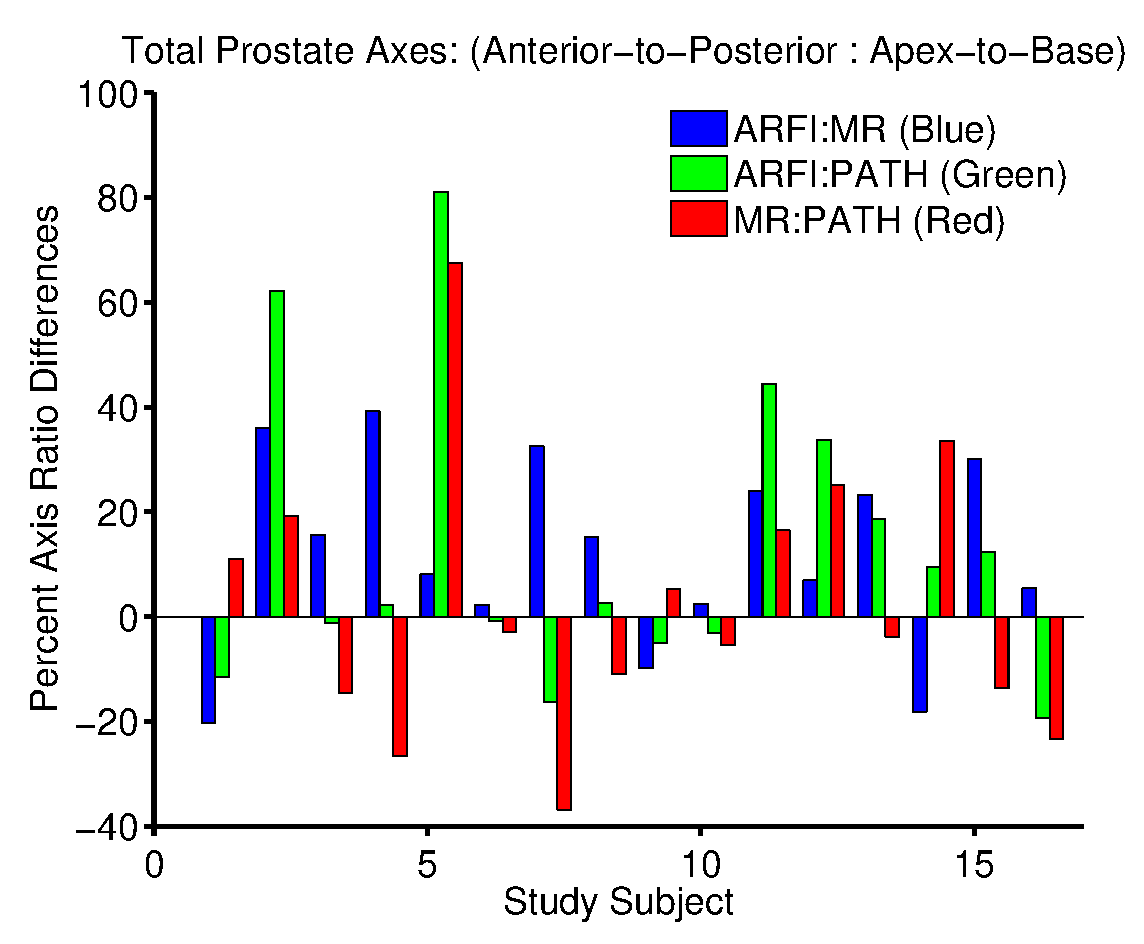
\includegraphics[width=0.3\linewidth]{figs/mr_arfi_total_over_under2} &
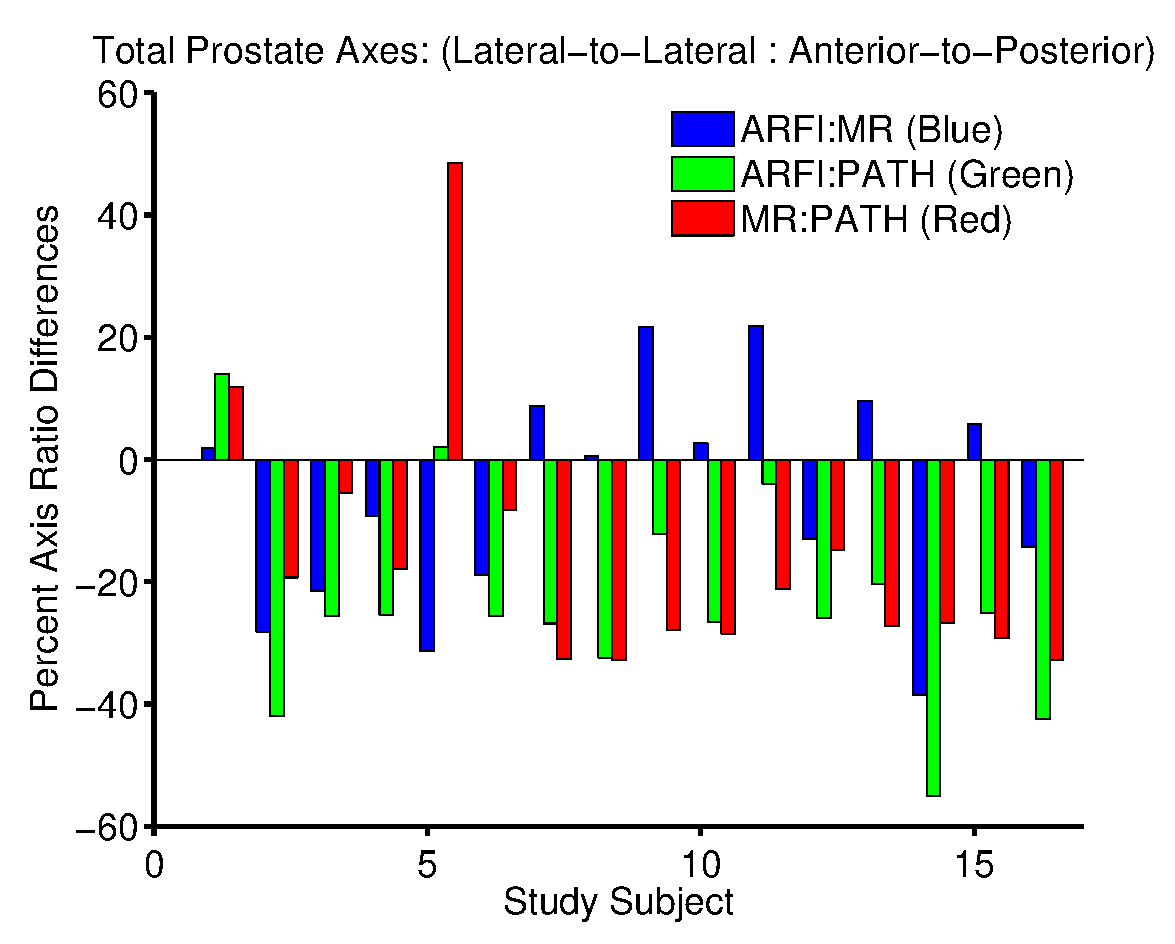
\includegraphics[width=0.3\linewidth]{figs/mr_arfi_total_over_under3} \\
(d) & (e) & (f) \\
\end{tabular}
\caption{Comparison of the ratios of the three anatomic axis measurement ratios
    for T2WI MR (top row, blue), ARFI imaging (top row, green) and gross
    pathology (top row, red).  The over/underestimation of the axis ratios
    between ARFI imaging : T2WI MR : Pathology are shown in the bottom row
    (d-f), with mean ratio differences compiled in
    Table~\ref{tab:axis_ratio_over_under}.}
\label{fig:mr_arfi_total_axes} 
\end{figure}


\begin{figure}
\centering
\begin{tabular}{ccc}
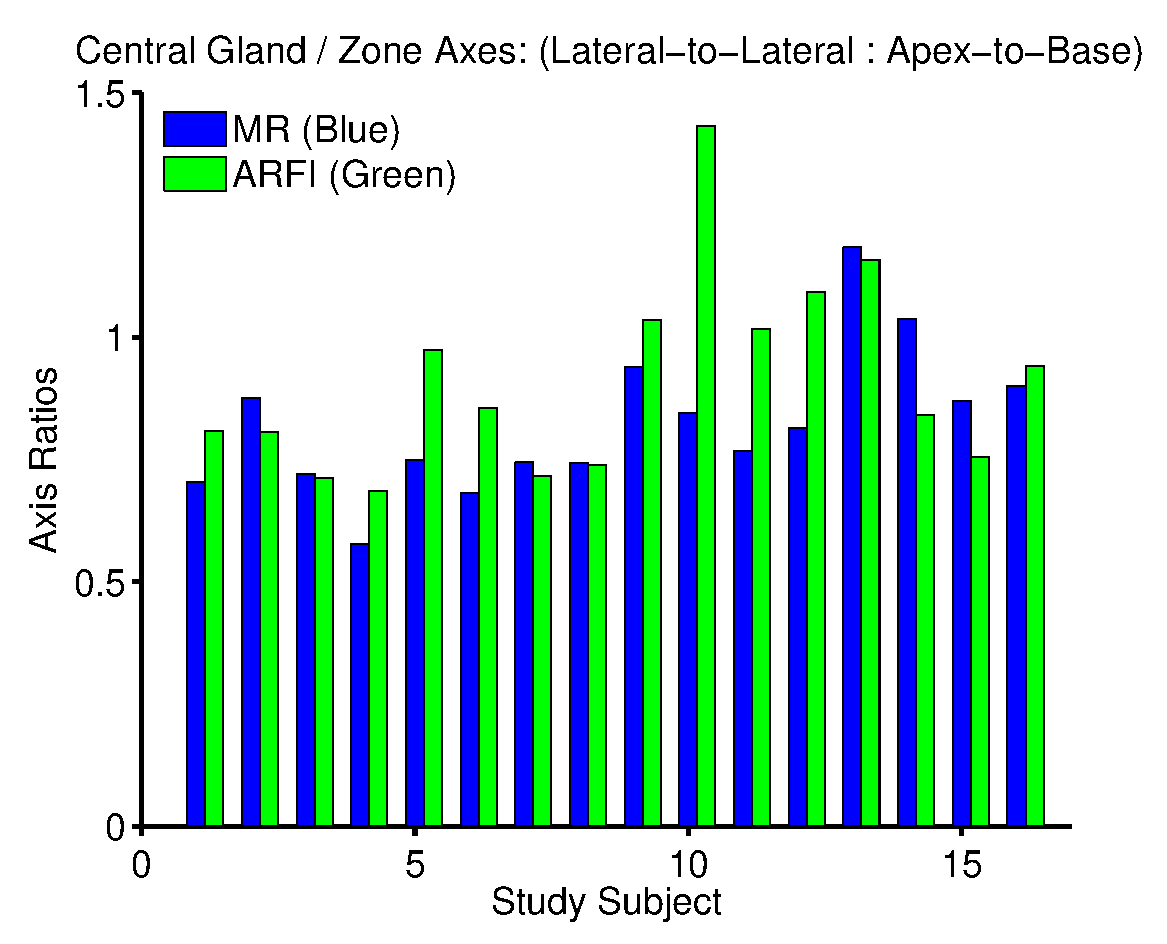
\includegraphics[width=0.3\linewidth]{figs/mr_arfi_central_axes1} &
\includegraphics[width=0.3\linewidth]{figs/mr_arfi_central_axes2} &
\includegraphics[width=0.3\linewidth]{figs/mr_arfi_central_axes3} \\
(a) & (b) & (c) \\
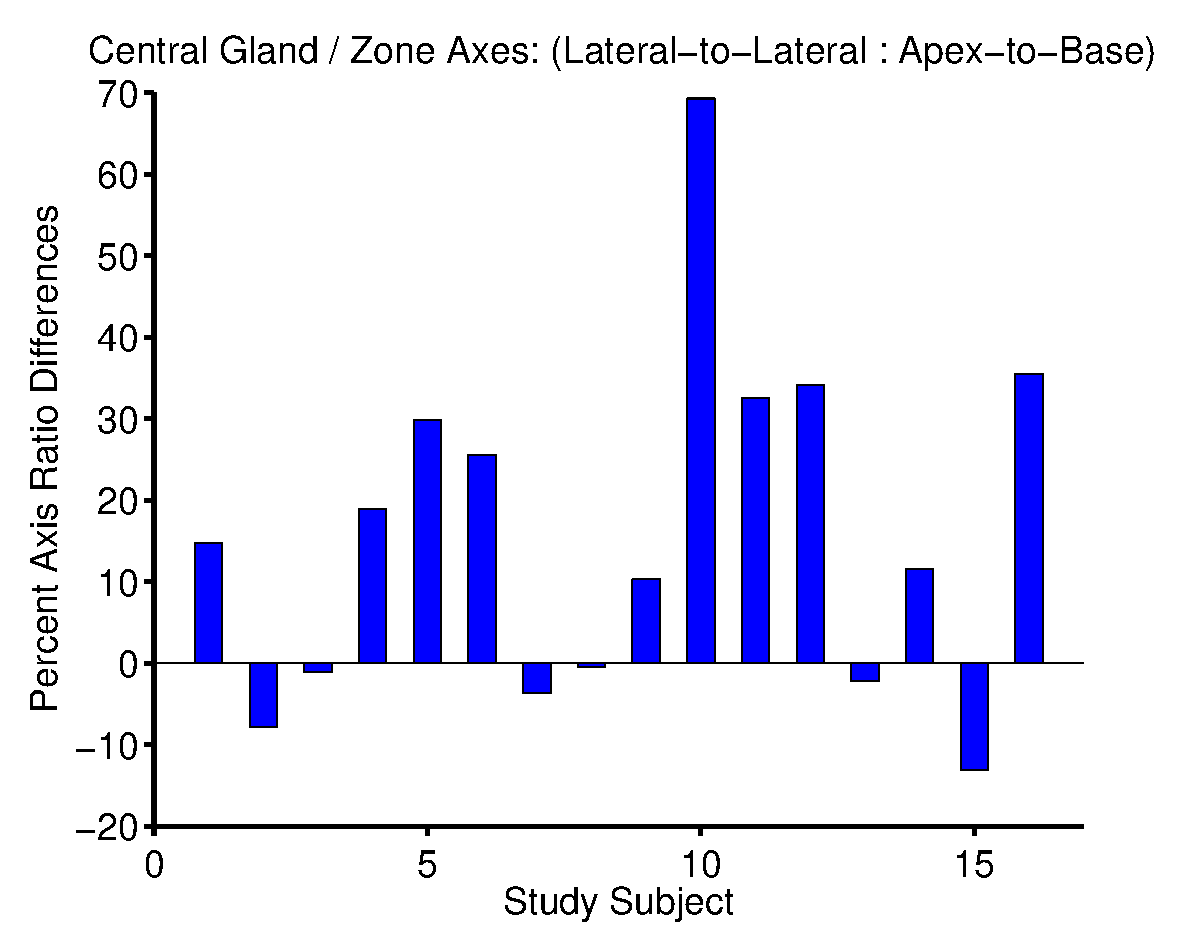
\includegraphics[width=0.3\linewidth]{figs/mr_arfi_central_over_under1.eps} &
\includegraphics[width=0.3\linewidth]{figs/mr_arfi_central_over_under2.eps} &
\includegraphics[width=0.3\linewidth]{figs/mr_arfi_central_over_under3.eps} \\
(a) & (b) & (c) \\
\end{tabular}
\caption{Comparison of the ratios of the three anatomic axis measurement ratios
    for T2WI MR (top row, blue) and ARFI imaging (top row, green).  The
    over/underestimation of the axis ratios between ARFI imaging and T2WI MR
    are shown in the bottom row (d-f), with mean ratio differences compiled in
    Table~\ref{tab:axis_ratio_over_under}.}
\label{fig:mr_arfi_central_axes} 
\end{figure}


\begin{table}
\centering
\caption{Mean axis ratio differences between ARFI imaging, T2WI MR and
    pathology for the total prostate volume and central gland / zone for the
    imaging modalities.  The three axis ratios analyzed were:
    lateral-to-lateral : apex-to-base (LL:AB), anterior-to-posterior :
    apex-to-base (AP:AB), and lateral-to-lateral : anterior-to-posterior
    (LL:AP).}
\begin{tabular}{|l|l|l|l|l|} \hline
{\bf Image Modality} & {\bf Comparative Measure} & {\bf Total / Central} & {\bf Axes} & {\bf Axis Ratio Difference (\%)} \\ \hline
ARFI & MR & Total & LL:AB & 13.9 $\pm$ 22.9 \\ 
ARFI & PATH & Total & LL:AB & 39.3 $\pm$  27.6 \\ 
MR & PATH & Total & LL:AB & 24.7 $\pm$ 26.0 \\ 
ARFI & MR & Total & AP:AB & 5.2 $\pm$ 22.6 \\ 
ARFI & PATH & Total & AP:AB & 5.4 $\pm$  28.3 \\ 
MR & PATH & Total & AP:AB & 2.5 $\pm$ 26.0 \\ 
ARFI & MR & Total & LL:AP & -6.4 $\pm$ 18.3 \\ 
ARFI & PATH & Total & LL:AP & -23.3 $\pm$  17.1 \\ 
MR & PATH & Total & LL:AP & -16.5 $\pm$ 21.1 \\ 
ARFI & MR & Central & LL:AB & 12.0 $\pm$ 22.5 \\ 
ARFI & MR & Central & AP:AB & -8.8 $\pm$ 20.8 \\ 
ARFI & MR & Central & LL:AP & -15.4 $\pm$ 25.9 \\ 

\hline
\end{tabular}
\label{tab:axis_ratio_over_under}
\end{table}

